\section{The modular group}

Throughout this section and also later, we adopt the notation of Schoeneberg \cite{schoeneberg1974elliptic}.

\begin{definition}
\label{dfn_ModularGroup}
\index{Modular!group}
\index{Modular!transformation}
\index{Inhomogeneous!modular transformation}
A M�bius transformation $\phi$ of the form
\begin{equation*}
\phi(z) = \moebius{a}{b}{c}{d}{z},\quad a,b,c,d \in \Z,\quad ad - bc = 1
\end{equation*}
is called \emph{(inhomogeneous) modular transformation}.
\end{definition}

\begin{theorem}
\label{thm_ModularGroup}
\index{Modular!group}
The set of modular transformations forms a discrete subgroup of the group of M�bius transformations and can be identified with the projective special linear group $\PSL{\Z}$. This group is called the \emph{modular group} and is denoted by $\ModGrp$.
\end{theorem}
\begin{proof}
The proof is very similar to that of Theorem \ref{thm_MoebiusGroup}. The only thing which has to be changed is the homomorphism $\pi$ defined in (\ref{eqn_homPi}). Its domain now is $\SL{\Z}$, the group of 2-by-2 matrices over $\Z$ with determinant 1, rather than $\GL{\C}$ (or $\SL{\C}$). Again it follows by the first isomorphism theorem, that the modular group $\ModGrp$ is isomorphic to $\SL{\Z} / \ker(\pi) \cong \PSL{\Z}$. The fact that $\ModGrp$ is a discrete subgroup of the group of M�bius transformations is now also directly evident.
\end{proof}

\begin{remark}
\index{Inhomogeneous!modular transformation}
\index{Homogeneous!modular transformation}
\index{Modular!transformation}
The elements of $\SL{\Z}$ are often called \emph{homogeneous modular transformations}, whereas the transformations of $\ModGrp = \PSL{\Z}$ are called \emph{inhomogeneous}. Strictly seen, an inhomogeneous transformation has to be denoted as $[M]_{\sim}$, which is the equivalence class in $\PSL{\Z}$ of a matrix $M \in \SL{\Z}$. It is clear, that $[M]_{\sim}$ is nothing but the set $\{\pm M\}$ and again for easier notation, we will from now on simply write either $M$ or $-M$ instead of $[M]_{\sim}$.
\end{remark}

\todo{16}{Basic mapping properties}

\subsection{Generators and relations}

In group theory it is an important question, which systems of group elements and relations (in the sense of definition \ref{dfn_GrpConstructGenRel}) completely describe the structure of any given group. This section is devoted to the answer of this question in the case of the modular group.

Before we start, we introduce the following modular transformations which will serve as group generators:

\begin{IEEEeqnarray*}{RL}
U: & z \mapsto z + 1 \\
T: & z \mapsto -\reci{z} \\
R = TU: & z \mapsto -\reci{z + 1}
\end{IEEEeqnarray*}

\begin{remark}
Sadly, in literature there is no consensus about the notation of these transformations. We use the notation of Schoeneberg \cite{schoeneberg1974elliptic} here, but other notations are frequent. In Klein/Fricke \cite{klein1966vorlesungen}, the symbol $S$ is used instead of $U$ and in other literature as well as on Wikipedia, additionally the roles of $S$ and $T$ are swapped.
\end{remark}

\begin{theorem}
\label{thm_ModGrpGen}
The modular group is generated by the elements $U: z \mapsto z+1$ and $T: z \mapsto -\reci{z}$. 
\end{theorem}
\begin{proof}
Let $A: z \mapsto \moebius{a}{b}{c}{d}{z}$ be an arbitrary modular transformation. Our goal is to show that $A$ can be written as product of the transformations $U$ and $T$. For this purpose it is more convenient to view these transformations as elements of $\PSL{\Z}$, namely
\begin{equation*}
A = \mat{a}{b}{c}{d}, \quad U = \mat{1}{1}{0}{1}, \quad T = \mat{0}{-1}{1}{\phantom{+}0}.
\end{equation*}

Let's first consider the two special cases, when $a$ or $c$ are zero. If $a=0$, it follows from $ad - bc = 1$, that $-b = c = \pm 1$.  Therefore we have
\begin{equation*}
A \sim c A = \mat{0}{-1}{1}{c d} = TU^{c d}.
\end{equation*}
Similarly, $c = 0$ gives $a = d = \pm 1$ and
\begin{equation*}
A \sim a A = \mat{1}{a b}{0}{1} = U^{a b}.
\end{equation*}
In the general case, when $a$ and $c$ are both nonzero, $ad - bc = 1$ implies that $a$ and $c$ are coprime and the Euclidean algorithm therefore yields
\begin{eqnarray*}
      a &=& q_0 \cdot c\phantom{_0} + r_1 \\
      c &=& q_1 \cdot r_1 + r_2 \\
    r_1 &=& q_2 \cdot r_2 + r_3 \\
        &\vdots& \\
r_{n-1} &=& q_n \cdot r_n + r_{n+1}\\
        &=& q_n \cdot 1\phantom{_n} + 0.
\end{eqnarray*}
We can use this to reduce the Matrix $A$ by successively multiplying powers of $U$ and $T$ from the left. Just note, that multiplication with $U^k$ adds $k$ times the second row to the first row, whereas $T$ swaps the rows and changes the sign of one arbitrary row\footnote{This freedom of choice is again due to the fact that the matrices $M$ and $-M$ represent the same element in $\PSL{\Z}$.}. If we concentrate only on the first column of $A$ and apply the first few transformations
\begin{equation*}
\cvec{a}{c}                           \overset{U^{-q_0}}{\longmapsto}
\cvec{r_1}{c\phantom{_1}}             \overset{T}{\mapsto} 
\cvec{\phantom{+}c\phantom{_1}}{-r_1} \overset{U^{q_1}}{\longmapsto}
\cvec{\phantom{+}r_2}{-r_1}           \overset{T}{\mapsto} 
\cvec{r_1}{r_2}                       \overset{U^{-q_2}}{\longmapsto}
\cvec{r_3}{r_2}                       \overset{T}{\mapsto}
\cvec{\phantom{+}r_2}{-r_3}           \mapsto \dots,
\end{equation*}
we soon recognize the general mapping rule, which is
\begin{IEEEeqnarray*}{rCll}
\cvec{\phantom{+}r_{j-1}}{\phantom{+}r_{j\phantom{+0}}} 
& \overset{TU^{-q_j}}{\longmapsto}
& \cvec{\phantom{+}r_{j\phantom{+0}}}{-r_{j+1}}
& \quad \text{for even } j \text{ and}\\
\cvec{\phantom{+}r_{j-1}}{-r_{j\phantom{+0}}}
& \overset{TU^{q_j}}{\longmapsto}
& \cvec{\phantom{+}r_{j\phantom{+0}}}{\phantom{+}r_{j+1}} 
& \quad \text{for odd } j.
\end{IEEEeqnarray*}
When we set $r_{-1} := a$ and $r_0 := c$, this rule is true for $0 \le j \le n$. Obviously the described procedure ends with
\begin{equation*}
\cdots \overset{T}{\mapsto}
\cvec{\phantom{+}r_{n\phantom{+0}}}{\pm r_{n+1}} = \cvec{1}{0}.
\end{equation*} 
Because we know the first column of the resulting matrix and its determinant, which is 1, we can conclude that for some $k \in \Z$ it must have the form
\begin{equation*}
\mat{1}{k}{0}{1} = U^k.
\end{equation*}
By setting $e_n := (-1)^{n} q_n$, we therefore have 
\begin{equation*}
TU^{-e_n} TU^{-e_{n-1}} \cdots TU^{-e_1}TU^{-e_0} A = U^k
\end{equation*}
or equivalently,
\begin{equation*}
A = U^{e_0} TU^{e_1} \cdots TU^{e_{n-1}} TU^{e_n} T U^k,
\end{equation*}
which gives the desired representation of $A$ in terms of $U$ and $T$ in the case when $a$ and $c$ are both non-zero.
\end{proof}

It is worth formulating the algorithm used in the previous proof explicitly in the following corollary.
\begin{corollary}
\label{cor_ModGrpTUAlg}
An arbitrary modular transformation $A: z \mapsto \moebius{a}{b}{c}{d}{z}$ can be represented in terms of the transformations $U: z \mapsto z+1$ and $T : z \mapsto -\reci{z}$, by performing the following steps:
\begin{enumerate}
\item If $a = 0$, then $A = TU^{c d}$ and if $c = 0$, then $A = U^{a b}$ and we are done. Otherwise, continue with \ref{itm_ModGrpTUAlgStart}.
\item \label{itm_ModGrpTUAlgStart} Apply the Euclidean algorithm to $a$ and $c$ with the first division being $a = q_0 \cdot c + r_1$ ($q_0$ may be $\le 0$) and let $n$ be the number of the  last division (start counting from 0). Call the arising quotients $q_0,q_1,\dots,q_n$.
\item For $j \in \{0,1,\dots,n\}$ set $e_j := (-1)^j q_j$.
\item Calculate the matrix product $TU^{-e_n} TU^{-e_{n-1}} \cdots TU^{-e_1}TU^{-e_0} A$ and multiply by $\pm 1$ in order to obtain a representation with positive diagonal elements. Read off the right-upper entry and call it $k$.
\end{enumerate}
The transformation $A$ can now be written as
\begin{equation}
\label{eqn_ModGrpTUAlg}
A = U^{e_0} TU^{e_1} \cdots TU^{e_{n-1}} TU^{e_n} T U^k.
\end{equation}
\end{corollary}

We have seen that $U$ and $T$ generate the modular group, but it is not yet clear, which group words in $U$ and $T$ give the same modular transformations. For example, it is easy to see that $T^2 = 1$ and $(TU)^3 = 1$ are relations satisfied by $T$ and $U$. Before we can show, that these two relations are ``the only ones'', \ie all other relations can be derived from them, we need the following Lemma:

\begin{lemma}
Let $a, b, c, d \in \Z$ be arbitrary integers satisfying $ad - bc = 1$. Then one, and only one of the following three conditions is true:
\begin{IEEEeqnarray*}{RRCCCRCC}
  (i)\quad & ac       &\ge& 0 &\quad\land\quad&       bd &\ge& 0\\
 (ii)\quad & a^2 + ac &\le& 0 &\quad\land\quad& b^2 + bd &\le& 0\\
(iii)\quad & c^2 + ac &\le& 0 &\quad\land\quad& d^2 + bd &\le& 0
\end{IEEEeqnarray*}
\end{lemma}
\begin{proof}
It is trivial to see, that $(i)$ implies $\lnot (ii)$ and $\lnot (iii)$. It therefore remains to show, that $\lnot(i)$ implies either $(ii)$ or $(iii)$.
\end{proof}

\begin{theorem}
\label{thm_ModGrpRel}
The generators $T: z \mapsto -\reci{z}$ and $R: z \mapsto -\reci{z+1}$ of the modular group satisfy the relations
\begin{equation}
\label{eqn_ModGrpTRRel}
T^2 = \id{\C}, \quad R^3 = \id{\C}
\end{equation}
and all other relations are derived from these two. Therefore the modular group is isomorphic to the free product of a cyclic group of order 2 and a cyclic group of order 3.
\end{theorem}

\todo{18}{Proof}

% ------------------------------- Subsection: Fundamental domains, tessellation
\subsection{The fundamental domain and the tessellation of the halfplane}

\begin{figure}
\centering
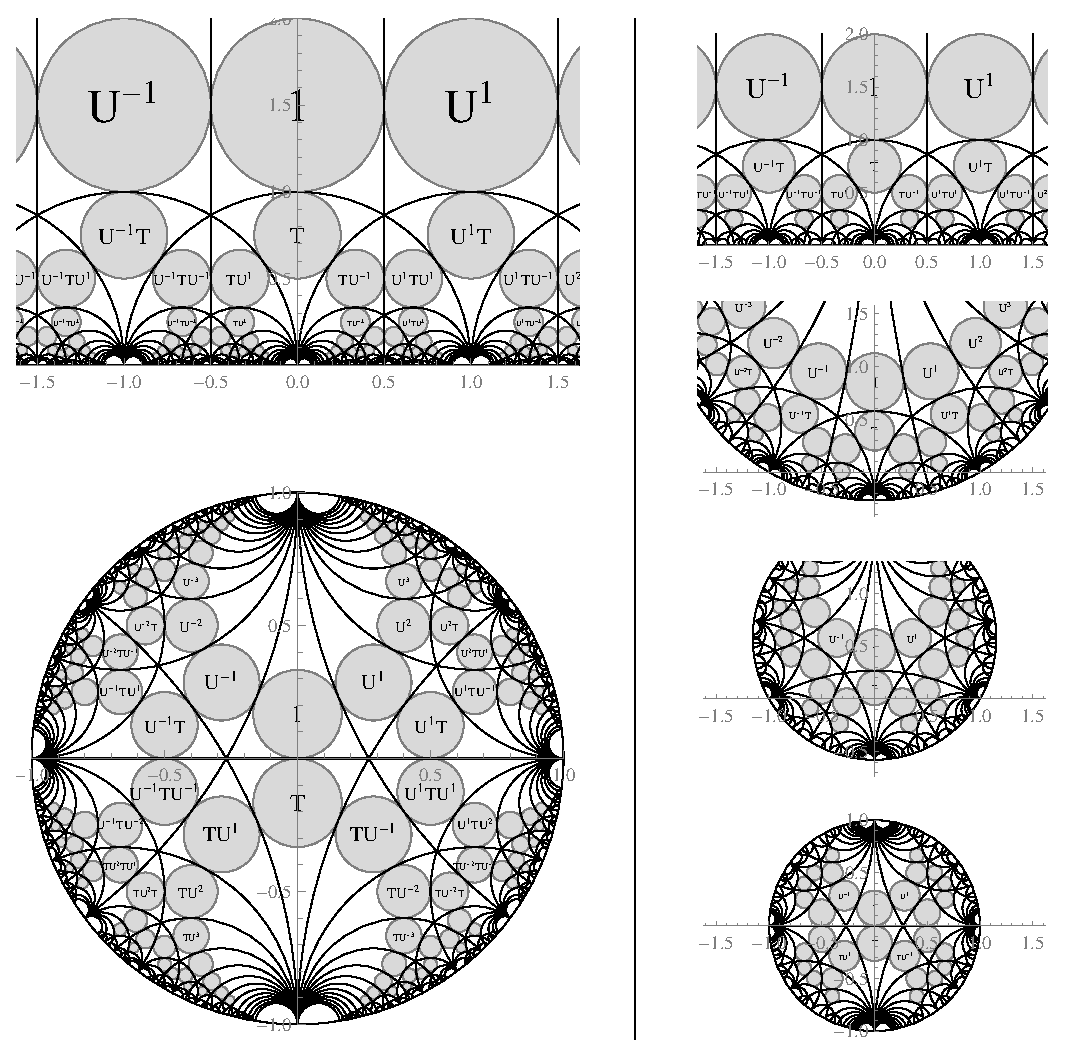
\includegraphics[width=\textwidth]{figures/modular-tiling-1}
\caption{The tessellation of the upper halfplane.}
\label{fig_ModularTiling}
\end{figure}


\todo{25}{Definition, description and figures}


% --------------------------------------------- Subsection: Hyperbolic geometry
\subsection{Hyperbolic geometry}

\todo{11}{Connection to hyperbolic geometry (disk/halplane model)}


% ------------------------------- Subsection: Ford circles, continued fractions
\subsection{Ford circles and continued fractions}

For an arbitrary modular transformation $A$, a representation as product of shifts $U^j: z \mapsto z+j$ and inversions $T: z \mapsto -\reci{z}$ can be found by the algorithm described in Corollary \ref{cor_ModGrpTUAlg}. By writing out this product, for example in the case when $n=2$, we have
\begin{equation*}
A = U^{e_0}T U^{e_1}T U^{e_2}T U^k,
\end{equation*}
or more explicitly
\begin{equation}
\label{eqn_ALongConFrac}
A(z) = e_0 - \reci{e_1 - \reci{e_2 - \reci{k + z}}}.
\end{equation}
\index{Continued fraction}
Here, a close relation between modular transformations and continued fractions immediately gets apparent. In this section we will investigate this relation somewhat deeper. 
First, we will use Pringsheim's more space-saving notation for continued fractions, namely
\begin{equation}
\label{eqn_ConFracNotation}
b_0 + \frac{a_1}{b_1 + \frac{a_2}{b_2 + \frac{a_3}{b_3 + \dots}}} =: 
b_0 + \cfr{a_1}{b_1} + \cfr{a_2}{b_2} + \cfr{a_2}{b_3} + \dots
\end{equation}
In the case when all $a_j = 1$, we adhere to the standard sequence notation for continued fractions:
\begin{equation*}
b_0 + \reci{b_1 + \reci{b_2 + \dots}} =: [b_0,b_1,b_2,\dots].
\end{equation*}
We can now reformulate Corollary \ref{cor_ModGrpTUAlg} in order to construct a continued fraction representation of any given modular transformation.

\begin{corollary}
An arbitrary modular transformation $A(z) = \moebius{a}{b}{c}{d}{z}$ can be written as continued fraction
\begin{equation}
\label{eqn_ModTransConFrac}
A(z) = [q_0,q_1,\dots,q_n,(-1)^{n+1}(k+z)]
\end{equation}
where the integers $n$, $q_0,q_1,\dots,q_n$ and $k$ are determined by the algorithm described in Corollary \ref{cor_ModGrpTUAlg}.
\end{corollary}
\begin{proof}
By using the continued fraction representation of $A$ given in (\ref{eqn_ALongConFrac}) and by applying the definition $e_j$ := $(-1)^j q_j$ we see
\begin{IEEEeqnarray}{rCcCcCcCcCcCc}
A(z) &=& e_0 &+& \cfr{-1}{e_1} 
          &+& \cfr{-1}{e_2} 
          &+& \dots 
          &+& \cfr{-1}{e_n} 
          &+& \cfr{-1}{k + z} \nonumber \\
  &=& q_0 &+& \cfr{-1}{-q_1} 
          &+& \cfr{-1}{q_2} 
          &+& \dots 
          &+& \cfr{-1}{(-1)^n q_n} 
          &+& \cfr{-1}{k + z}. \label{eqn_ModTransConFracInterim}
\end{IEEEeqnarray}
Now for every odd $j \le n$ we can rewrite 
\begin{equation*}
\cfr{-1}{-q_j} + \cfr{-1}{\dots} \quad \text{to} \quad \cfr{1}{q_j} + \cfr{1}{\dots}.
\end{equation*}
Thus if $n$ is odd, every numerator $-1$ in (\ref{eqn_ModTransConFracInterim}) can be turned into $+1$. In the other case, when $n$ is even, only one negative numerator at the end, $\frac{-1}{k+z}$, remains, but this can easily be rewritten to $\frac{1}{-(k+z)}$. Taking both cases together, we obtain (\ref{eqn_ModTransConFrac}).
\end{proof}

\begin{figure}
\centering
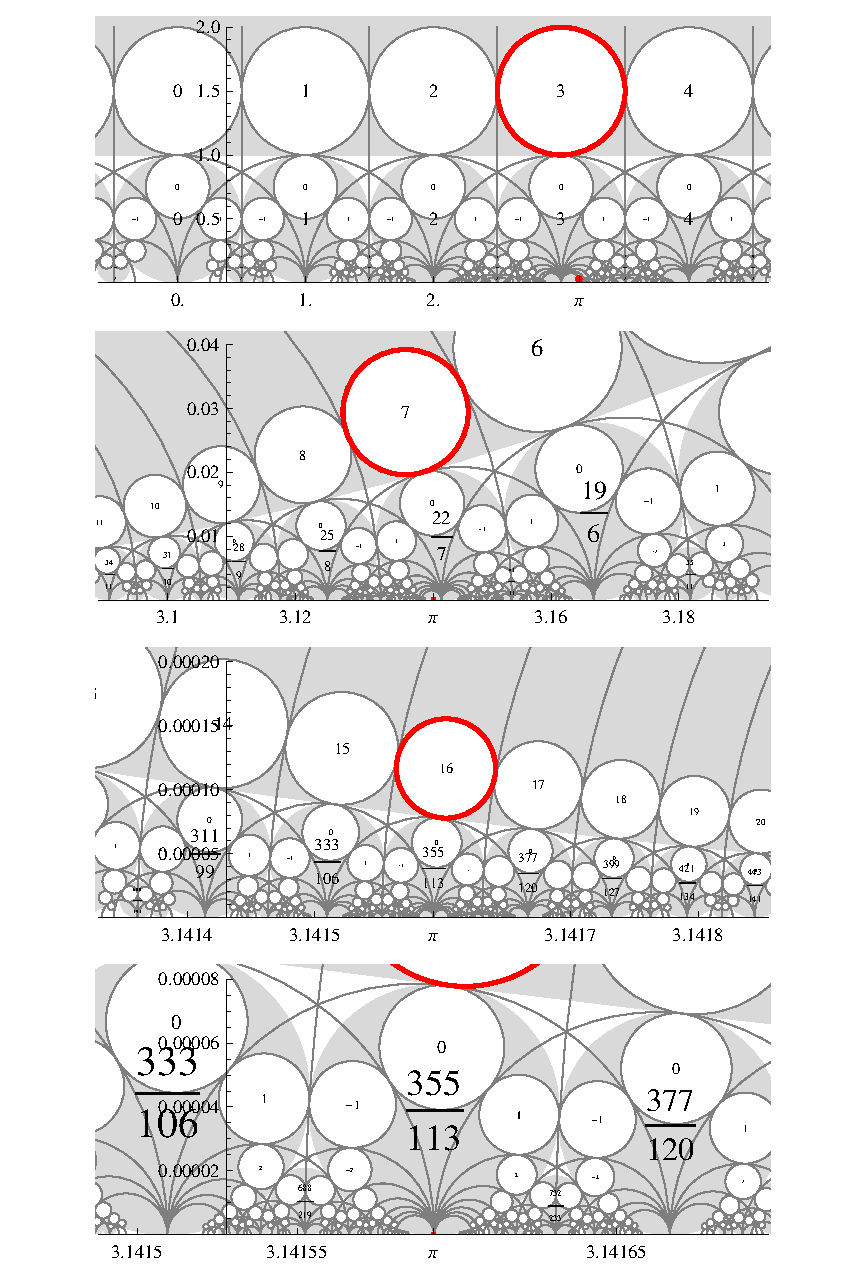
\includegraphics[width=\textwidth]{figures/cont-frac-pi}
\caption{$\pi = \frac{355}{113}$ -- well, almost.}
\label{fig_ContFracPi}
\end{figure}


\todo{19}{The modular group and ford circles}


